%===================================
%===================================
%===================================
\setchapterpreamble[u]{\margintoc}
\chapter{Combined cooling pilot plant at Plataforma Solar de Almería}
\labch{cc:facility}

\tldrbox{ In this chapter a detailed description of the combined cooling pilot
    plant at \gls{psaLabel} is provided including a \gls{pYidLabel} diagram and
    the methodology followed to perform the experimentation and data-processing.
    Several experimental campaigns have been performed to characterize the
    different components of the pilot plant and the complete system, at a wide
    range of operating conditions. Combined, 198 tests are processed most of
    which are openly available in public repositories. }

\section*{Introduction}

The combined cooling pilot plant at Plataforma Solar de Almería is a unique
facility that integrates a wet cooling tower and a dry cooler in a flexible
hydraulic configuration. It allows for the study and validation of different
cooling configurations, models, and control and optimization strategies.

% Historia de la planta
\todo{Historia de la planta}

This chapter describes the
plant in \nrefsec{cc:facility:description} and the experimental campaigns carried
out in \nrefsec{cc:facility:exp}.

% TODO: A la salida de la segunda válvula hay que añadir una flecha para que
% sea más legible, renombrar válvulas V1 y V2 a Vp y Vs.
\begin{figure*}[h!]
	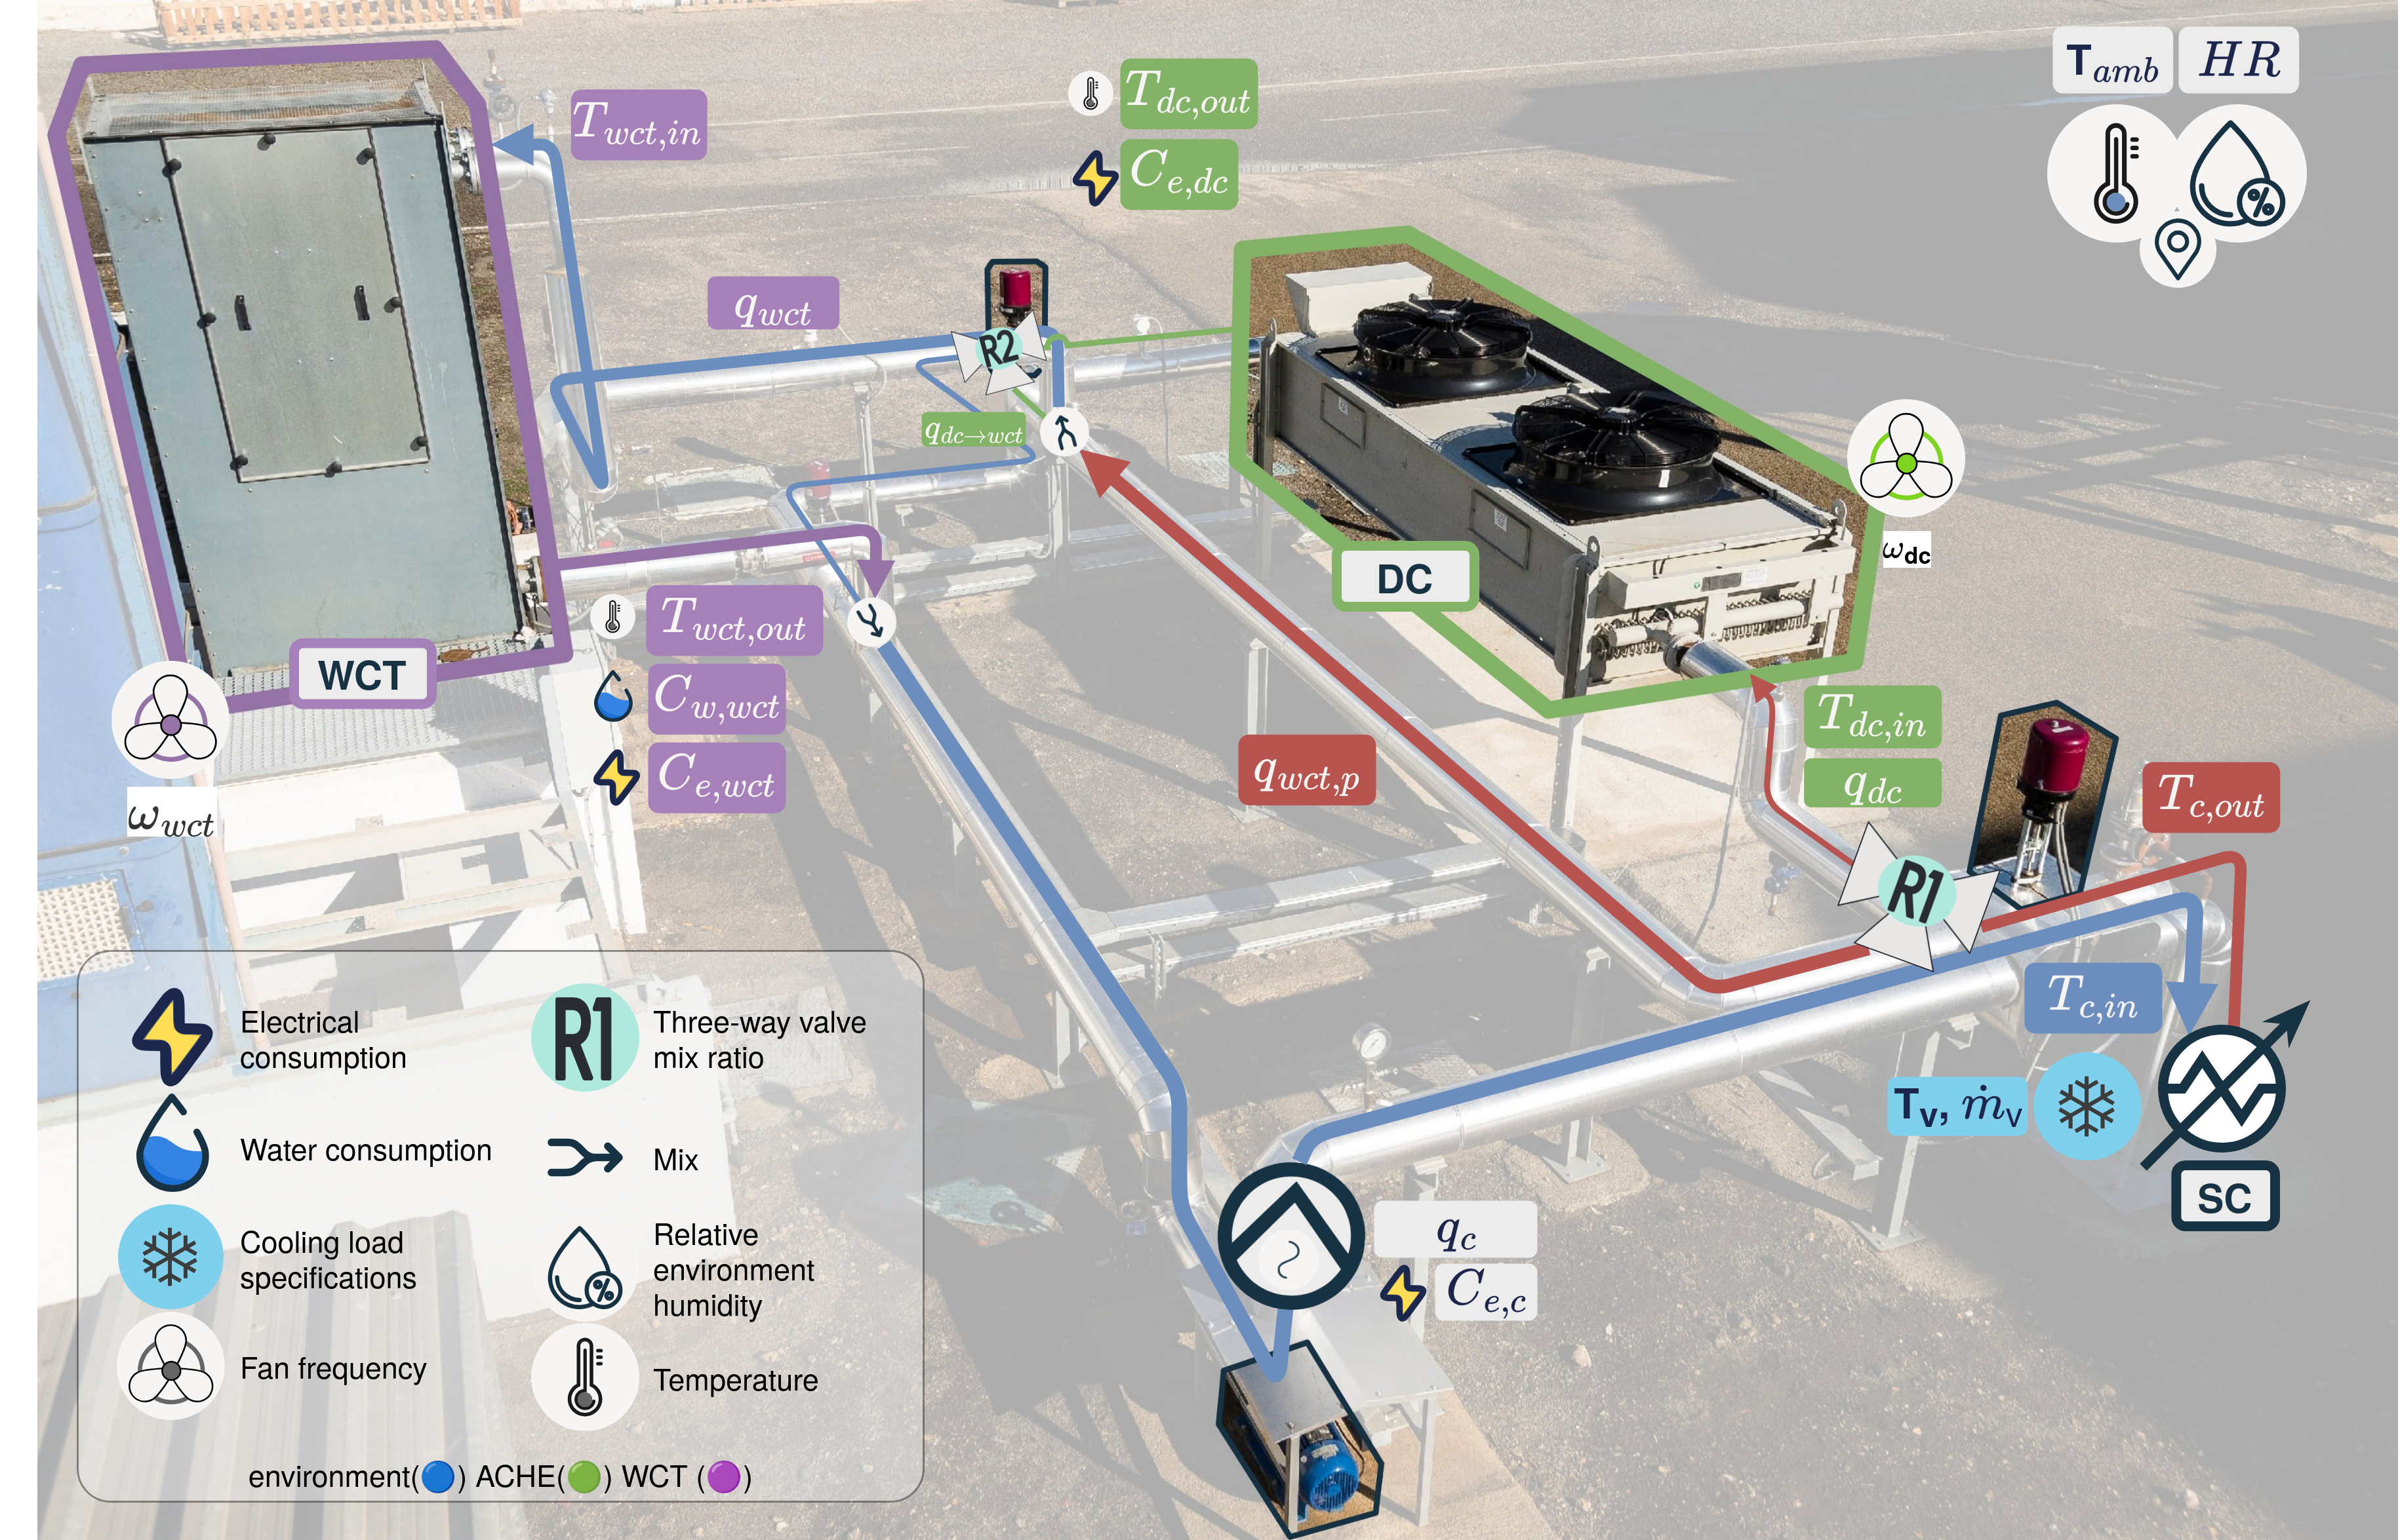
\includegraphics[]{figures/WASCOP-facility-diagram.png}
	\caption{\gls{psaLabel} combined cooling system facility}
	\labfig{cc:facility:cc-pilot-plant-diagram}
\end{figure*}


%===================================
%===================================
\section{Plant description}
\labsec{cc:facility:description}

% Sacado de: Wet cooling tower performance prediction in \gls{cspLabel} plants:
% A comparison between artificial neural networks and Poppe’s model
The pilot plant of combined cooling systems located at \gls{psaLabel} (see the
layout in \reffig{cc:facility:pid}) consists of three circuits:
cooling, exchange and heating. In the cooling circuit (see a picture in
\reffig{cc:facility:wct-back-view}), water circulating inside the tube bundle of
a Surface Condenser (\gls{scLabel}) can be cooled through a Wet Cooling Tower and/or a Dry
Cooling Tower (type Air Cooled Heat Exchanger, \gls{acheLabel}), both with a designed
thermal power of 204~kW$_{th}$. In the exchange circuit, a saturated steam
generator of 80~kW$_{th}$ (on the design point), generates steam at different
pressures (in the range between 82~mbar and 200~mbar), which is in turn
condensed in the surface condenser. In this way, the steam transfers its latent
heat of condensation to the refrigeration water, that is heated. Finally, in
the heating circuit, a solar field with a thermal power of 300~kW$_{th}$ at the
design point, provides the energy required by the steam generator, in the form
of hot water. It is a unique, very flexible, fully instrumented and versatile
facility, able to operate in different operation modes: series and parallel
mode, conventional dry-only mode (all water flow is cooled through the dry
cooling tower) and wet-only mode (all water flow is cooled through the wet
cooling tower). The instrumentation related to the \gls{wctLabel} is described in
\reftab{cc:facility:instr}. 

Note that sensors measuring the air velocity, temperature and relative humidity
at the outlet area of the wet cooling tower are not permanently installed in the
plant. Portable sensors were used instead in some experiments to characterize
them. They were measured at the outlet area of the cooling tower\sidenote{Using
the sensors listed in \reftab{cc:facility:instr}}. The outlet area was divided
into 9 quadrants and the above mentioned magnitudes were registered at the
center of each quadrant. The obtained values were averaged to determine the mean
velocity, temperature and relative humidity used in the air mass flow rate
calculation. 


\begin{marginfigure}[-7cm]
    \includegraphics[]{figures/WASCOP-facility-WCT.png}
	\caption{Back view of the \gls{wctLabel}}
    \labfig{cc:facility:wct-back-view}
\end{marginfigure}

In regards to operational aspects of the system, note that the cooling water
and air flow rates at the experimental facility ($\dot{m}_w$, and air,
$\dot{m}_a$, respectively), are modified with the \textit{Pump 1} and the fan
frequency percentage \texttt{\gls{scLabel}-001}, respectively (see
\reffig{cc:facility:pid}).

\begin{table}[h]
\caption{Characteristics of instrumentation ($^a$ value of the temperature in $^\circ$C, $^b$ of reading, $^c$ full scale, $^d$ mean value).} 
\labtab{cc:facility:instr}
\resizebox{\linewidth}{!}{
\begin{tabular}{cccc} 
    \toprule
    \textbf{Measured variable} & \textbf{Instrument} & \textbf{Range}  &
    \textbf{Measurement uncertainty}\\
    \midrule
    Water temperature & Pt100 & 0 - 100 $^\circ$C & 0.03 + 0.005$\cdot T^a$\\
    (\texttt{TT-001}... \texttt{TT-007}) & & &\\
    Cooling water flow rate & Vortex flow meter & 9.8 - 25 m$^3$/h & $\pm$ 0.65
    \% o.r.$^b$\\
    (\texttt{FT-001}...\texttt{FT-003})  & & &\\
    Water flow rate  & Paddle wheel & 0.05 - 2 m$^3$/h & $\pm$ 0.5 \% of
    F.S$^c$  \\
    (\texttt{FT-004}) & flow meter  & & + 2.5 \% o.r\\
    Condensate water & Coriolis flow meter & 0.1 - 0.3 m$^3$/h & $<$ 0.1  \% \\
    flow rate  (\texttt{FT-006}) &   & & + \\
    
    Ambient temperature & Pt1000 & -40 - 60 $^\circ$C  & $\pm$ 0.4 $@$20
    $^\circ$C \\
    Relative humidity & Capacitive sensor & 0 - 98\% & $\pm$ 3 \% o.r $@$20
    $^\circ$C  \\
            Air velocity & Impeller anemometer & 0.1-15$~\mbox{m s$^{-1}$}$ &
            $\pm$ 0.1$~\mbox{m s$^{-1}$}$ + 1.5 \%  o.r \\
            Outlet air temperature & Pt100   & -20-70$^\circ$C & $\pm
            0.5^\circ$C \\
            Outlet air humidity & Capacitive sensor   & 0-100\%& $\pm$ 2\% \\
    \bottomrule
\end{tabular}
}
\end{table}

\begin{figure}
    \includegraphics[width=1\textwidth]{figures/WASCOP-facility-PID.png}
    \caption{Layout of combined cooling systems pilot plant at \gls{psaLabel}.}
    \labfig{cc:facility:pid}
\end{figure}


%===================================
%===================================
\section{Experimental campaigns}
\labsec{cc:facility:exp}

With the aim of characterizing and developing models for this novel facility,
over the years several experimental campaigns have been carried out.

The normative framework followed to carry out the experiments, in order to
ensure stable conditions, has been the standards \texttt{UNE
13741}~\sidecite{une_thermal_2004a} and the Spanish
CTI~\sidecite{cti_code_2000}. These standards specify the test duration and the
allowed variations of the most representative ambient and operating magnitudes
(water flow rate, heat load, cooling tower range, wet-bulb and dry-bulb
temperatures and wind velocity) during the tests. Although the duration of the
test should not be less than one hour according to the standards, due to the low
capacity of the \gls{wctLabel} in the PSA pilot plant and the operational experience, the
duration of the tests has been reduced to up to 30 minutes. Once stable
conditions are maintained during the defined interval time, the average and
deviations values of each measurement are calculated in order to check that they
are within the allowable limits of the norm, which finally lead to a valid
steady-state operating point. 

\section{Wet cooling tower}
\labsec{cc:facility:exp-wct}

A total of 132 steady-state experimental points have been obtained. These data
cover a large variety of ambient conditions (different seasons, days and
nights) and thermal loads (from 27 to 207 kW). The objective of the
experimental campaigns is to develop and validate two modelling strategies for
the performance evaluation of the \gls{wctLabel}\sidenote{See
\nrefsec{cc:modelling:wct}}.

% \reffig{cc:facility:example-test} shows the main variables involved in one of
% the experiments performed at the pilot plant at constant air flow rate
% ($f_{fan}$=25~\%). As can be observed, there are two time intervals in this
% case, in which the process is at stationary conditions according to the
% normative framework mentioned. In order to process the results of the
% experimental tests and identify valid time intervals, such as the ones shown in
% this example, a function has been implemented in the \textit{MATLAB}
% environment. This function identifies whether the standard criteria is met and
% calculates the mean values of the required variables.

% \begin{figure}
%     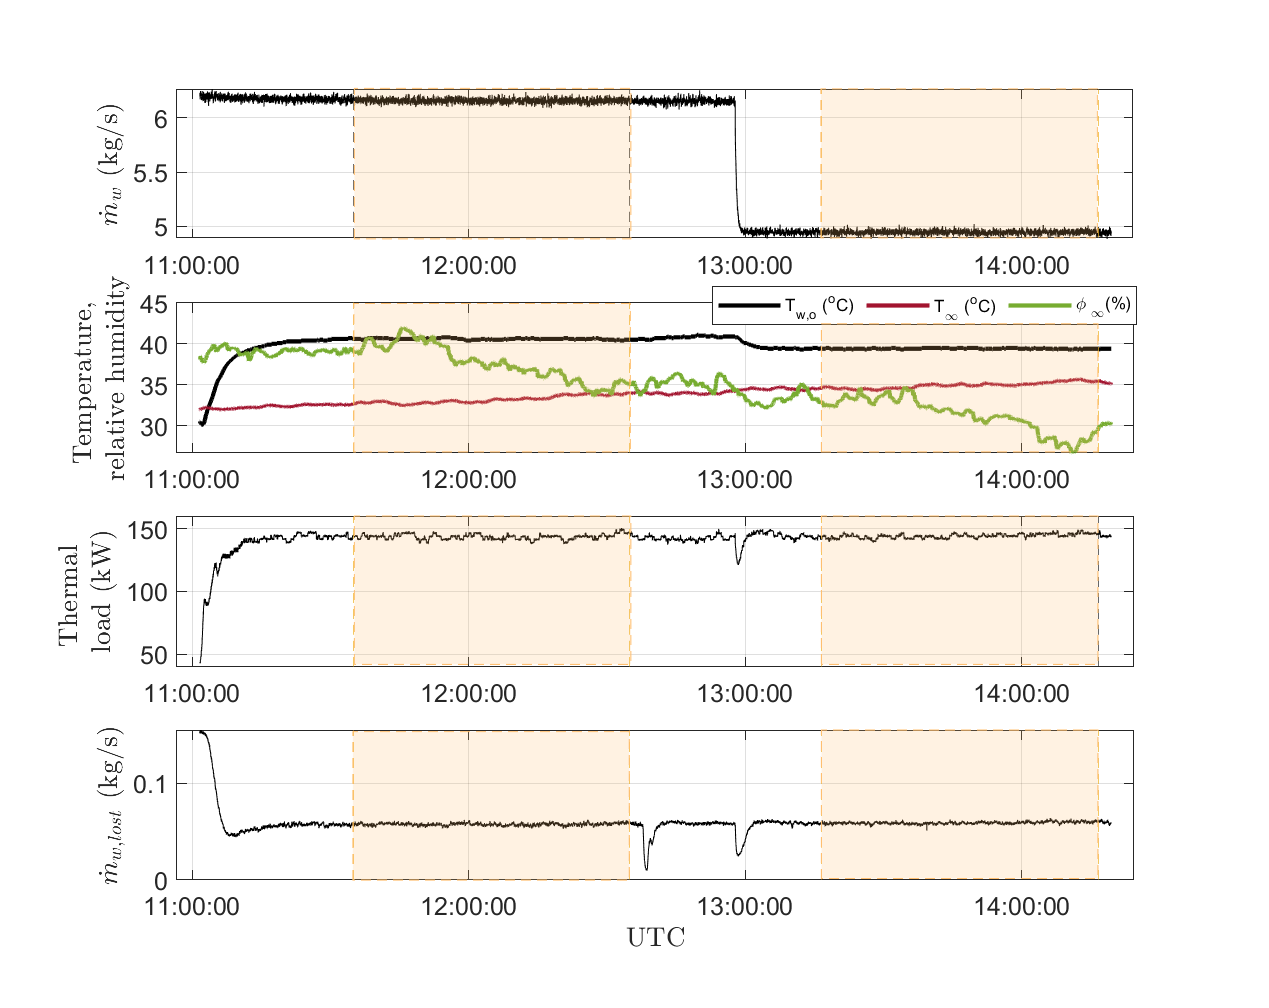
\includegraphics[]{figures/wascop-test-220726.eps}
%     \caption{Example of one experiment at the pilot plant in July with two
%     valid steady-state operating points.} 
%     \labfig{cc:facility:example-test}
% \end{figure}

The data from the different experimental campaigns is available at
\sidecite{palenzuela_steadystate_2024a,serrano_wet_2024}.


%===================================
\subsection{Physical model calibration -- Exp 1}[Exp 1] 
\labsec{cc:facility:exp:1}

The experimental campaign was designed to calibrate the physical model by
focusing on the Merkel number, which depends on the water-to-air mass flow
ratio. A total of 19 tests were carried out at the PSA combined cooling pilot
plant, covering a wide range of water and air flow conditions. Water flow rates
varied from 8 to 22~m$^3$/h (2.17--6.15~kg/s), while air flow rates ranged from
1.16 to 4.32~kg/s by adjusting the fan frequency between 25~\% and 100~\%. Air
velocity, temperature, and humidity maps were measured at eight fan
levels\sidenote{This enables the calculation of the air mass flow rate at the
outlet of the cooling tower, $\dot{m}_a$, using the permanent sensors installed
in the facility}. Tests were performed under consistent summer conditions, with
high ambient temperatures (32--41~$^\circ$C) and low relative humidities
(13--40~\%).

%===================================
\subsection{Data-driven models training -- Exp 2}[Exp 2] 
\labsec{cc:facility:exp:2}

The data required for data-driven models depends on several factors such as the
complexity of the model and the error allowed or the diversity of the inputs.
With the aim of obtaining a reliable model for the \gls{wctLabel}, data collected
over several years of operation of the combined cooling system have been used
for tuning. They are a set of 115 stationary data covering the following
operating ranges: ambient temperature, $T_\infty$, \mbox{[9-39] $^{\circ}$C},
ambient humidity, $\phi_\infty$, [10-87] \%, inlet water temperature,
$T_{w,i}$ [33-41] $^\circ$C, cooling water flow rate, $q_w$, [6-23] $m^3/h$
and fan frequency percentage, $f_{fan}$ [21-94]~\%. The thermal load in these
tests varies in the range of [27-178]~${kW}_{th}$. The number of steady-state
data obtained is a reasonable value when compared to other similar data-driven models of
counter-flow cooling towers, as in the case of
\cite{hosoz_performance_2007}, where 81 experimental points
were collected for training and testing.

%===================================
\subsection[Experimental campaign 3]{Validation -- Exp 3}[Exp 3] 
\labsec{cc:facility:exp:3}

With the aim of validating and comparing different modelling approaches, a
dataset of 17 tests (different from the ones taken for experimental campaigns 1
and 2) has been compiled. This experimental campaign was designed using a
design of experiments based on full factorial design with 4 factors and 2
levels (low and high), whose values are shown in
\reftab{cc:facility:exp:3:doe}.  

\begin{margintable}[*-5]
    \caption{Design of experiments for model comparison (Exp 3)} 
    \labtab{cc:facility:exp:3:doe} 
    \resizebox{\linewidth}{!}{
    \begin{tabular}{cccc} 
        \toprule Variable & Low level & High level  \\
        \midrule $T_{b}$ ($^{\circ}$C) & $\leq$ 10 & $\geq$ 15 \\
        $T_{w,i}$ ($^{\circ}$C) & $\leq$ 37 & $\geq$ 39 \\
        $\dot{m}_w$ (kg/s) & $\leq$ 3.3 & $\geq$ 5 \\
        $T_{w,i}-T_{w,o}$ ($^{\circ}$C)  & $\leq$ 7 & $\geq$ 8 \\
        \bottomrule 
    \end{tabular}
    }
\end{margintable}

% An additional test at design operating conditions of the \gls{wctLabel}
% (\mbox{$T_{b,\infty}$=21 $^{\circ}$C}, $T_{w,i}$=40 $^{\circ}$C,
% $\dot{m}_w$=6.9 kg/s and $T_{w,i}-T_{w,o}$=7 $^{\circ}$C) has been also
% included in this test campaign, where $T_{b,\infty}$ is the ambient wet bulb
% temperature and $T_{w,o}$ the temperature of the water at the outlet of the
% \gls{wctLabel}. 


%===================================
%===================================
\subsection{Dry cooler, Surface condenser and Combined cooler models}
\labsec{cc:facility:exp-others}

\reftab{cc:exp-campaigns} summarizes the experimental campaigns,
describing the \gls{doeLabel} employed and indicating the number of
tests conducted under steady-state conditions. The ranges of the variables
involved in the experiments are also indicated, with those used to define the
\gls{doeLabel} for each test campaign shown in bold.

\subsubsection{Dry cooler model -- \gls{dcLabel}-f, \gls{dcLabel}-cal, \gls{dcLabel}-val}
\labsec{cc:facility:exp:dc}

An experimental campaign (\reftab{cc:exp-campaigns} -- \textit{\gls{dcLabel}-cal}) was
designed and performed to calibrate the Nusselt number correlation as described
in Section \ref{sec:ache}. This campaign comprises 27 tests.

As air mass flow rate measurements are a specific requirement for the \gls{dcLabel} model,
the $\dot{m}_{air}$-$w_{dc}$ relationship was derived during an experimental
campaign (\reftab{cc:exp-campaigns} -- \textit{\gls{dcLabel}-f}). Air velocity and temperature were measured at 10
different fan speed levels, ranging from 11 \% to 100 \% in 10 \% increments.
The \gls{acheLabel} fan area was divided into eight quadrants, and measurements were taken
at the center of each quadrant. The recorded values were then averaged to obtain
the mean air velocity and temperature, which were used to calculate the air mass
flow rate.

\todo{campaña para modelo basado en datos??}

%================================
\subsubsection{Surface condenser model -- \gls{scLabel}-cal, \gls{scLabel}-val}
\labsec{cc:facility:exp:sc}

An experimental campaign (\reftab{cc:exp-campaigns} -- \textit{\gls{scLabel}-cal})  was designed and performed to
calibrate the global heat transfer coefficient, $U_c$, as a function of inlet
water temperature, $T_{c,in}$ and water flow rate, $q_{c}$. This campaign
comprises 15 tests.    

%================================
\subsubsection{Complete system validation -- CC-val}
\labsec{cc:facility:exp:cc}

An additional experimental campaign (\reftab{cc:exp-campaigns} --
\textit{CC-val}) was designed and performed to validate the complete model of
the \gls{ccLabel} system. This campaign comprises 24 tests.       


\begin{table}[]
\centering
\caption{Experimental campaigns performed at the \gls{ccLabel} pilot plant, where GD-n$_1$-n$_2$ refers to the spatial grid distribution ($n_1$) around the fan with $n_2$ measurements in each quadrant (\textit{$n_1 \times n_2$} measurements); \textit{BB-$n_1$-$n_2$} denotes a Box-Behnken design with \textit{$n_1$} variables and \textit{$n_2$} levels; and \textit{FF-$n_1$-...-$n_i$} indicates a full factorial design with \textit{$i$} variables, each with \textit{$n_i$} levels.}
\labtab{cc:exp-campaigns}
\resizebox{\textwidth}{!}{%
\begin{tabular}{rlccccccccccc}
\hline
\multirow{2}{*}{Features}              &  & \multicolumn{5}{c}{\textbf{Component calibration}}                                            & \multicolumn{1}{l}{} & \multicolumn{3}{c}{\textbf{Component validation}}           & \multicolumn{1}{l}{} & \textbf{System validation} \\ \cline{3-7} \cline{9-11} \cline{13-13} 
                                       &  & \gls{dcLabel}-f   & \multicolumn{1}{l}{} & \gls{dcLabel}-cal         & \multicolumn{1}{l}{} & \gls{scLabel}-cal            & \multicolumn{1}{l}{} & \gls{dcLabel}-val         & \multicolumn{1}{l}{} & \gls{scLabel}-val            & \multicolumn{1}{l}{} & CC-val                     \\ \cline{1-1} \cline{3-3} \cline{5-5} \cline{7-7} \cline{9-9} \cline{11-11} \cline{13-13} 
\gls{doeLabel}                                    &  & GD-8-10  & \multicolumn{1}{l}{} & BB-4-3           & \multicolumn{1}{l}{} & BB-3-3            & \multicolumn{1}{l}{} & BB-4-3           & \multicolumn{1}{l}{} & BB-3-3            & \multicolumn{1}{l}{} & FF-2-2-2-3                 \\
NumTests                               &  & 80       & \multicolumn{1}{l}{} & 27               & \multicolumn{1}{l}{} & 15                & \multicolumn{1}{l}{} & 27               & \multicolumn{1}{l}{} & 15                & \multicolumn{1}{l}{} & 24                         \\
$T_{amb}$ ($^\circ$C)                  &  & 26       &                      & \textbf{12 - 29} &                      & -                 &                      & \textbf{13 - 32} &                      & -                 &                      & \textbf{12 - 37}           \\
HR (\%)                                &  & -        &                      & -                &                      & -                 &                      & -                &                      & -                 &                      & 14 - 63                    \\
$\dot{m}_v$ (kg/h)                     &  & -        &                      & -                &                      & 118 - 328         &                      & -                &                      & 133 - 287         &                      & 200 - 310                  \\
$\dot{Q}_c$ (kW)                       &  & -        &                      & -                &                      & \textbf{78 - 216} &                      & -                &                      & \textbf{88 - 187} &                      & \textbf{132 - 202}         \\
$q_{c}$ (m$^3$/h)                      &  & -        &                      & -                &                      & \textbf{10 - 24}  &                      & -                &                      & \textbf{10 - 24}  &                      & \textbf{18 - 24}           \\
$q_{dc}$ (m$^3$/h)                     &  & -        &                      & \textbf{5 - 25}  &                      & -                 &                      & \textbf{5 - 24}  &                      & -                 &                      & \textbf{5 - 24}            \\
$q_{wct}$ (m$^3$/h)                    &  & -        &                      & -                &                      & -                 &                      & -                &                      & -                 &                      & \textbf{6 - 24}            \\
$T_{dc,in}$  ($^\circ$C)               &  & -        &                      & \textbf{35 - 41} &                      & -                 &                      & \textbf{31 -42}  &                      & -                 &                      & 33 - 54                    \\
$T_{dc,in}$ - $T_{dc,out}$ ($^\circ$C) &  & -        &                      & \textbf{2 - 7}   &                      &                   &                      & \textbf{2 - 9}   &                      &                   &                      & 1 - 11                     \\
$T_{v}$ ($^\circ$C)                    &  & -        &                      & -                &                      & \textbf{36 - 56}  &                      & -                &                      & \textbf{36 - 56}  &                      & \textbf{36 - 57}           \\
$T_{wct,in}$ ($^\circ$C)               &  & -        &                      & -                &                      & -                 &                      & -                &                      & -                 &                      & 33 - 54                    \\
$\omega_{dc}$ (\%)                          &  & 11 - 100 &                      & \textbf{11 - 76} &                      & -                 &                      & \textbf{11 - 98} &                      & -                 &                      & 11 - 100                   \\
$\omega_{wct}$ (\%)                         &  & -        &                      & -                &                      & -                 &                      & -                &                      & -                 &                      & 21 - 87         \\ \hline            
\end{tabular}%
}
\end{table}
